\section{Verification}
\label{sec:verification}

\subsection{Constitutive update}
The log-conformation update is verified against the analytic viscometric limits of
\cref{sec:constitutive}. Step-strain relaxation, steady simple shear (including the
first normal-stress difference $N_1$), and the elastic limit $\tau\to\infty$ are all
reproduced to machine precision:
\begin{center}\small
\begin{tabular}{@{}lll@{}}
\toprule
test & analytic target & error \\
\midrule
step-strain relaxation & $\sigma_{xy}=G\gamma e^{-t/\tau}$ & $\sim10^{-10}$ \\
steady shear & $\sigma_{xy}=G\tau\dot\gamma,\ N_1=2G\tau^2\dot\gamma^2$ & $\sim10^{-12}$ \\
elastic limit & $\be=\Ften\Ften^{\!\top}$ & $\sim10^{-13}$ \\
\bottomrule
\end{tabular}
\end{center}
With the exact relaxation substep \cref{eq:relax-exact} the step-strain response is
reproduced to machine precision at \emph{any} $\dt$, whereas the explicit update errs by
$0.29$ at $\dt/\tau=2$ and diverges by $\dt/\tau=5$. Positive-definiteness of $\be$ is
retained under extreme shear.

\subsection{Operators and projection}
The MAC divergence is exact on linear fields and second-order on smooth fields; the
identity $\mathrm{div}\circ\mathrm{grad}\equiv\mathrm{Lap}$ holds to $10^{-9}$; the
Poisson round-trip recovers the field to $10^{-10}$; and projecting an arbitrary
wall-boundary velocity yields divergence below $10^{-11}$ (machine-zero, the property the
collocated solver cannot reach). The FFT Helmholtz solve of \cref{eq:helmholtz} passes
the same round-trip to $10^{-10}$.

\subsection{Spatial order (all integrators)}
On the periodic Taylor--Green decaying vortex the solver is second order in space for
velocity, pressure and kinetic energy, and---crucially---the explicit, IMEX and
monolithic integrators produce \emph{identical} spatial errors at matched $\dt$
(\cref{fig:tg-conv}): the implicit and semi-Lagrangian machinery does not degrade spatial
accuracy. (For non-stiff advection the adaptive monolithic reduces to the central-%
difference IMEX, \cref{sec:monolithic}, so the three curves coincide.) The
implicit-viscosity scheme is additionally stable and accurate up to $\dt=50\times$ the
explicit viscous limit $\dx^2/(4\nu)$, where the explicit scheme diverges.

\begin{figure}[t]\centering
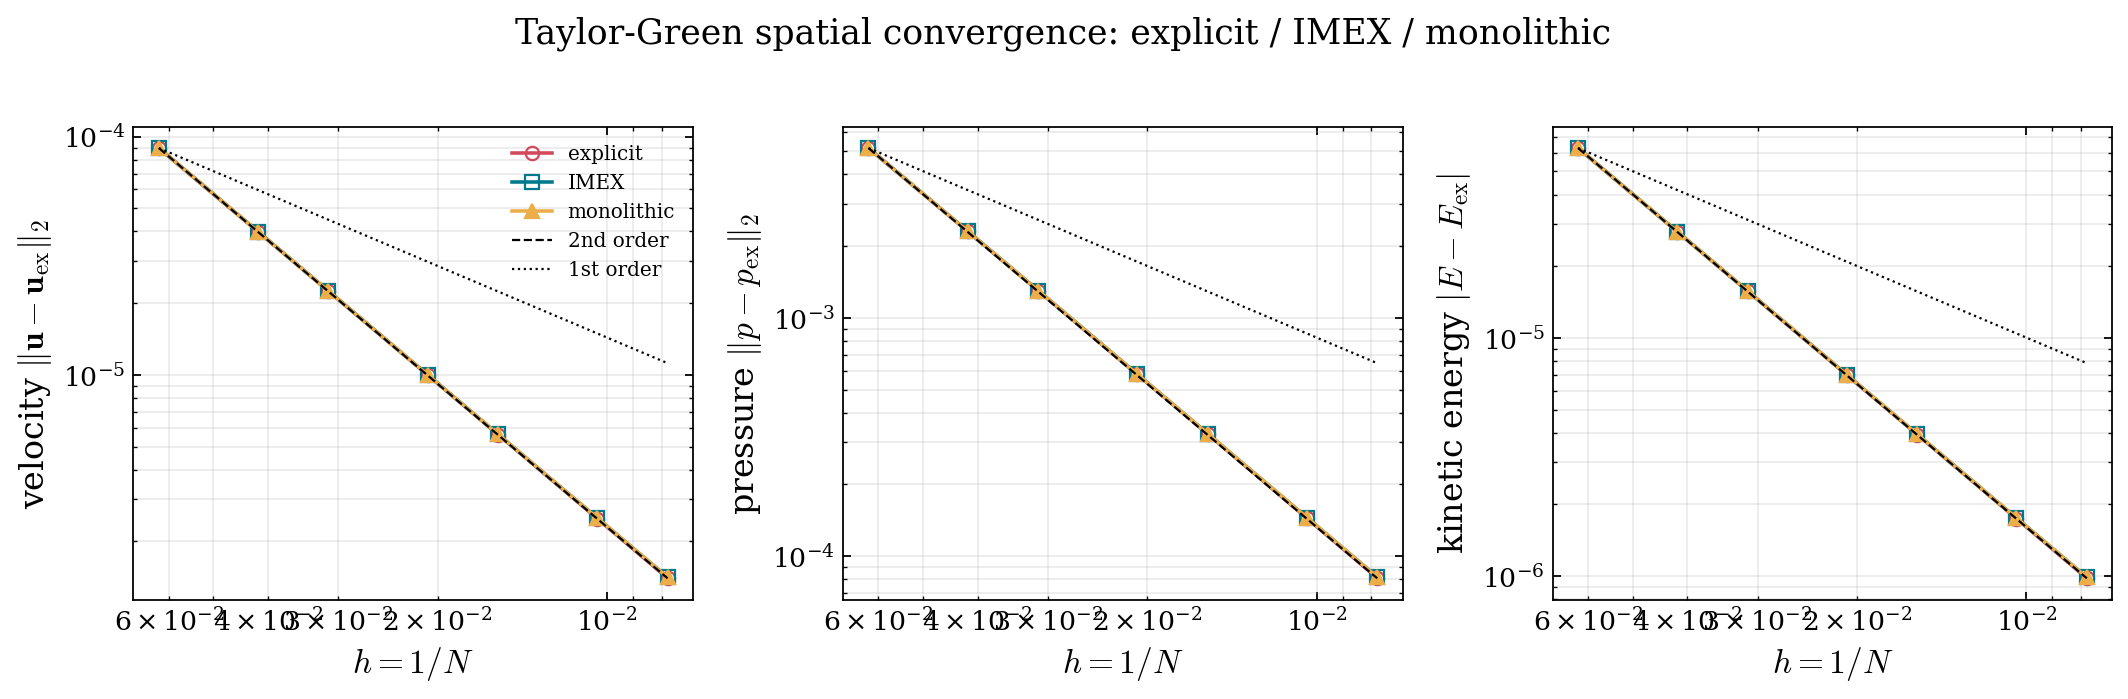
\includegraphics[width=\linewidth]{figures/tg_convergence_methods.png}
\caption{Taylor--Green spatial convergence of velocity, pressure and kinetic energy for
the explicit, IMEX and monolithic integrators (matched $\dt$). All three coincide on the
second-order reference line.}
\label{fig:tg-conv}
\end{figure}

\subsection{Energy conservation of the elastic coupling}
On the linear elastic standing shear wave the trapezoidal elastic coupling
(Proposition~\ref{prop:trap}) conserves the discrete energy across a wide range of time
steps, whereas the dissipative stage-1 stabilizer (Proposition~\ref{prop:vn}) damps the
wave away (drift $\to1$) and the explicit scheme diverges above the CFL:
\begin{center}\small
\begin{tabular}{@{}lccccc@{}}
\toprule
$\dt/\dt_{\rm CFL}$ & $0.5$ & $1$ & $2$ & $4$ & $8$ \\
\midrule
energy drift (5 periods) & $5.5\!\times\!10^{-5}$ & $2.2\!\times\!10^{-4}$ &
$1.8\!\times\!10^{-3}$ & $9.7\!\times\!10^{-3}$ & $9.6\!\times\!10^{-3}$ \\
\bottomrule
\end{tabular}
\end{center}
The drift stays below $1\%$ even at $8\times$ the explicit elastic CFL (the residual is the
$O(\dt^2)$ phase error of the resolved mode, not numerical dissipation). Separately, the
Oldroyd-B relaxation does not preserve $\det\be$: under steady shear the solver reproduces
the analytic $\det\be=1+\mathrm{Wi}^2$ (e.g.\ $1.36$ at $\mathrm{Wi}=0.6$), a bounded,
physical departure whose trace is carried by the pressure.
